%\documentclass{article}
%\usepackage{caption}
%\usepackage{graphicx}
%\begin{document}
\subsection*{}
In this section we will discuss about our mining algorithm \emph{USFP-growth}(algorithm-\ref{algorithm:mine}) That will find frequent patterns. For mining we used \emph{FP-growth} like approach. Generally, we can remove all the nodes having support less than \emph{minimum support}. From headr table we get such information that which nodes are less than \emph{minimum support}. We told earlier that for \emph{U\textsuperscript{cap}} value we took the upper limit, we also can we can remove all the nodes having prefix value less than \emph{minimum support}. In this process we can eliminate most of the infrequent nodes from tree. For this purpose we used header table that was created when creating the \emph{US-tree}. Then we construct conditional tree starting from the lowest support holding node. From header table we also get the position of all nodes containing same item in the tree. 
\subsection*{}
Lets mine the tree we constructed earlier. Figure-\ref{figure:min_before} is \emph{US-Tree} for mining and corresponding header table before starting mining. From the header table we get that support of \emph{a} is $3.00$, \emph{b} is $1.00$, \emph{c} is $3.30$, \emph{d} is $1.20$, \emph{e} is $0.60$. So \emph{e} is not frequent for one item set frequent pattern. So it is sure that no item set contains \emph{e} will be frequent. That is the basic upward closure property of frequent item set. So we remove all the nodes of \emph{e} and get the new mining tree Figure-\ref{figure:min_ready}. And its corresponding header. Here we find all one item sets that are frequent and that is \emph{\{a\}, \{b\}, \{c\} \{d\}} Now we will construct conditional tree for the found frequent one item and mine the conditional tree. But items having total \emph{U\textsuperscript{cap}} less than \emph{minimum support} is not needed to construct conditional tree because this \emph{U\textsuperscript{cap}} value has been take as the upper bound. So total \emph{U\textsuperscript{cap}} value less than \emph{minimum support} indicates that item must not be exists in the $2$ or more frequent item set. So we do not construct conditional tree for these items.
\subsection*{}
We construct conditional tree from items having lowest total \emph{U\textsuperscript{cap}} value greater than \emph{minimum support}. As \emph{b} having total \emph{U\textsuperscript{cap}} is $.69$ \emph{b} is ignored for constructing conditional tree. Then the next candidate is \emph{d}. From header table pointer we find that there is only one path item \emph{d} exists in the mining tree Figure-\ref{figure:min_ready}. That is \{\emph{a, c, d}\}:$1.08$. So we create conditional tree and update all nodes mining probability with \emph{d's} \emph{U\textsuperscript{cap}} $1.08$. For this conditional tree Figure-\ref{figure:d_cond} the header tables says all the nodes in the tree are having \emph{U\textsuperscript{cap}} greater than \emph{minimum support} $.9$. So all the items are ready to be constructed as conditional tree. As here is only one branch so we do not further construct conditional tree and take all the combinations as frequent items Figure-\ref{figure:d_cond} Table. so we find \emph{\{dc\}, \{da\}, \{dca\}} as frequent pattern. Next we create conditional tree for \emph{c}. Here c exists in the tree for three path those are \emph{\{a, c\} : $0.72$ , \{a , b, c\} : $.027$ and \{b, c\} : $0.27$}. So we create conditional tree (Figure-\ref{figure:c_cond}). Total mining value of \emph{c} is the sum of item caps in each respective path of \emph{c}. From the header we see that  \emph{b} has total cap having less than \emph{minimum support} so we remove \emph{b} and create two item set \emph{\{ca\}}. Next we construct \emph{ca} conditional tree that contains only root (\emph{\{\}}). So no further tree is needed to be constructed and minned. Than we create conditional tree for \emph{a}. And find only root \emph{\{\}}. Thus we get all the  frequent patterns. All the patterns are \emph{\{a\}, \{b\}, \{c\} \{d\}, \{dc\}, \{da\}, \{dca\} and \{ca\}}. As we have found all patterns from upper bound, so that it is guaranteed that there will be no false negative. But some false positive can be exists in the found frequent item set as there may be some value less than max value we assumed. so in the next section we will show an approach that eliminates the all false positives (if exists) in the data set.
%\documentclass{article}
%\usepackage{caption}
%\usepackage{graphicx}
%\begin{document}

\begin{figure}
\begin{minipage}{0.40\textwidth}
  \centering
  
	\begin{center}
	\begin{tabular}{ |c|c|c| } 
 	\hline
 		Item&\emph{U\textsuperscript{cap}}&Support\\ \hline\hline
 		a &  3.00  & 3.00	\\ \hline
 		c &  1.26  & 3.30	\\ \hline
 		d &  1.08  & 1.20	\\ \hline
 		e &  0.54  & 0.60	\\ \hline
 		b &  0.69  & 1.00	\\ \hline
\end{tabular}
\end{center}   
  \captionof{table}{Header Table of US-tree}
\end{minipage}
\hfill
\begin{minipage}{0.40\textwidth}
  \centering
  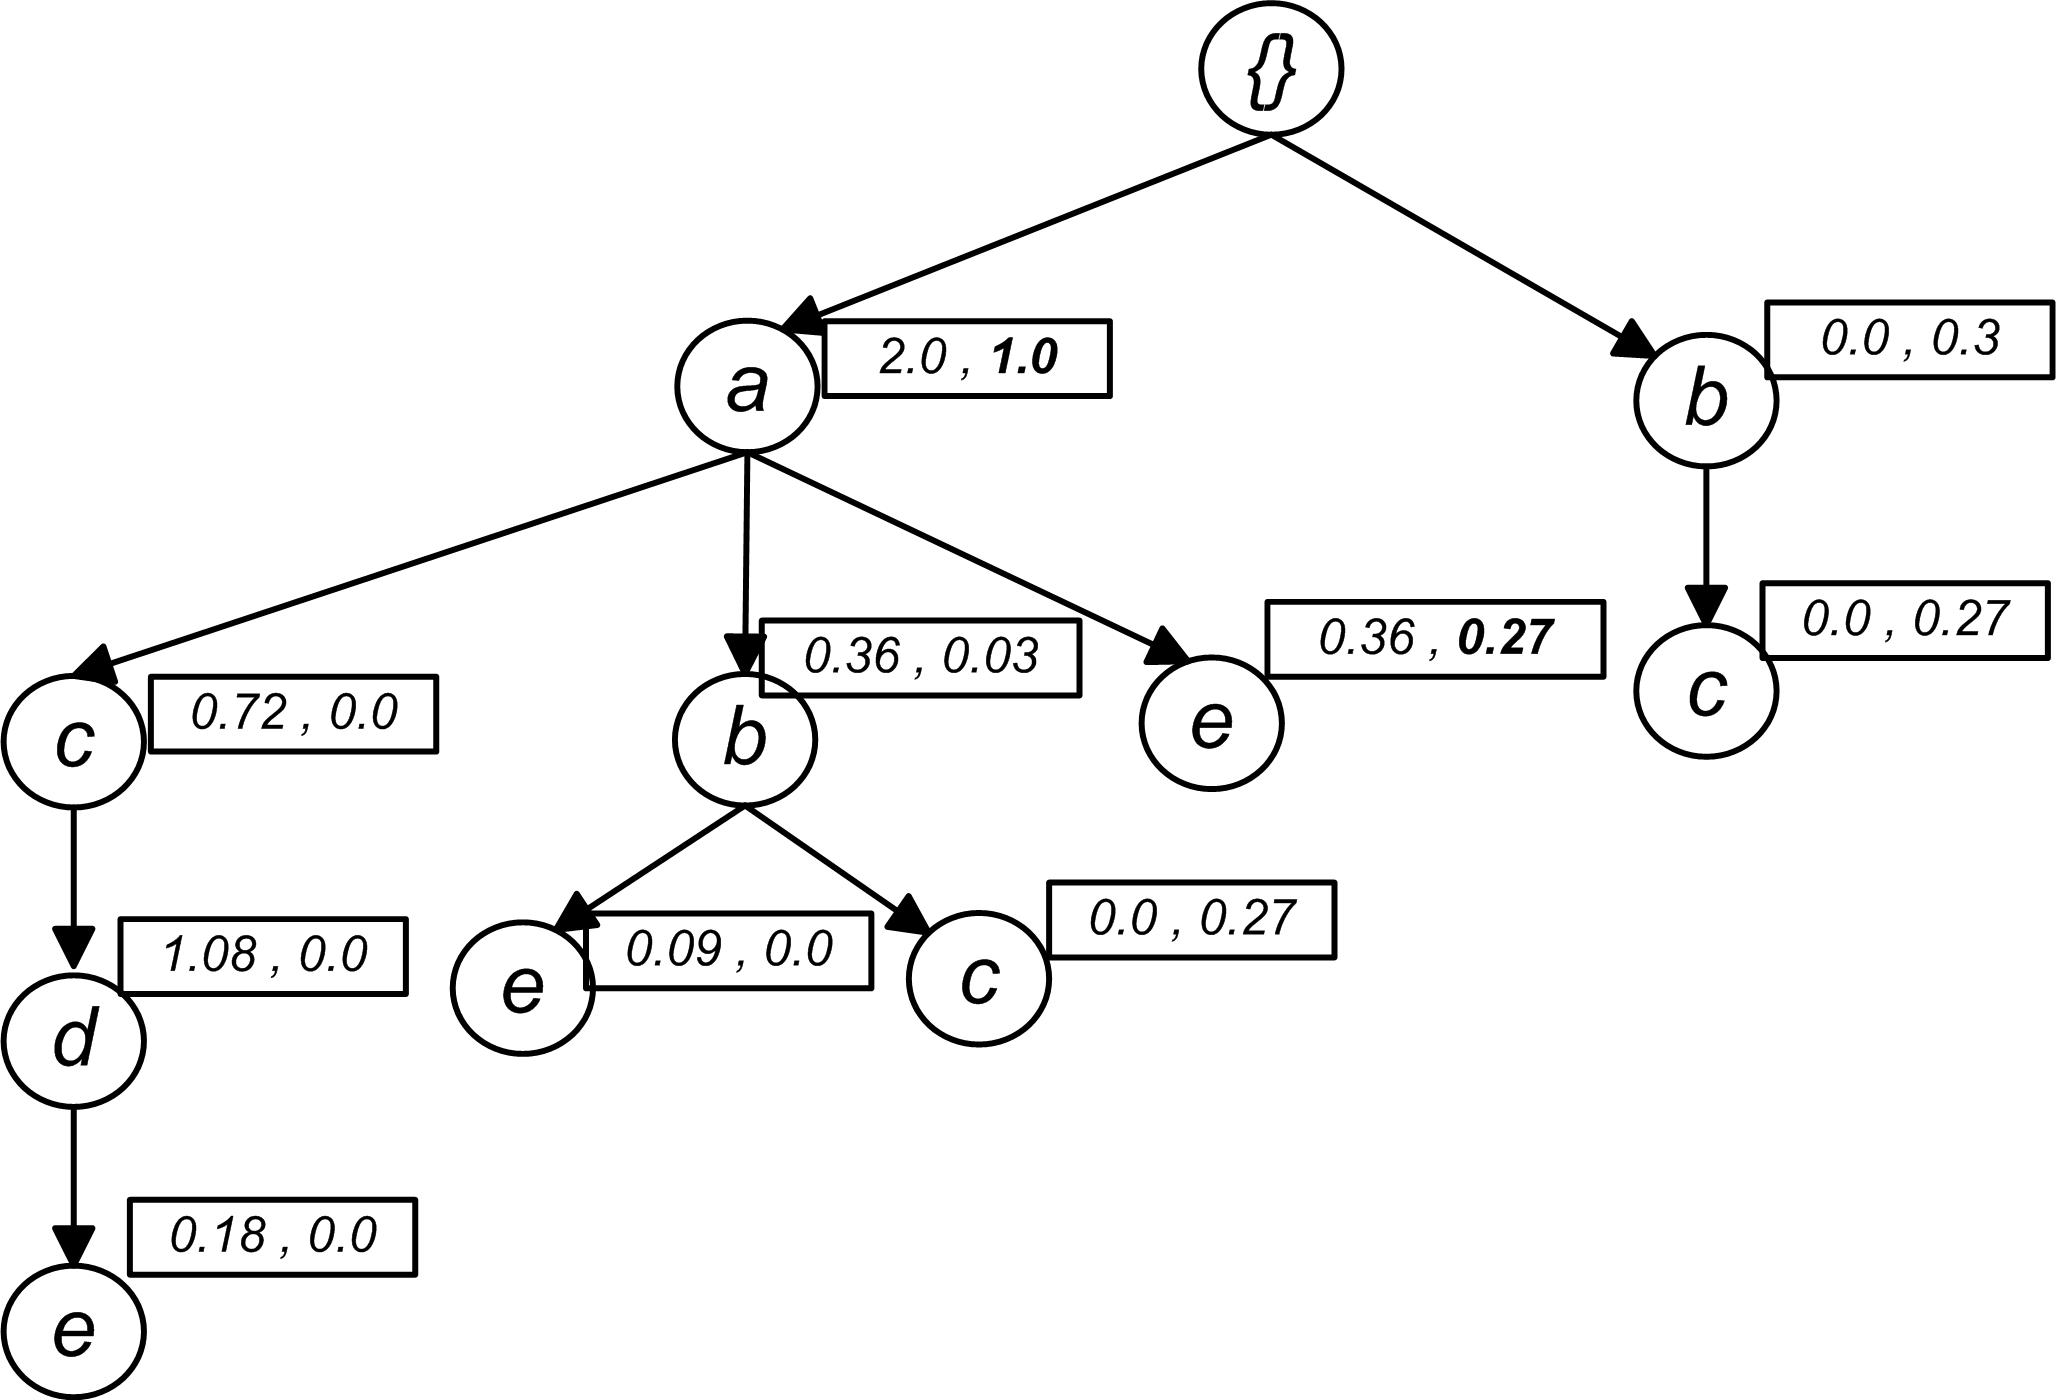
\includegraphics[width=\textwidth]{images/us_tree.jpg}
  \captionof{figure}{US-tree}
\end{minipage}
\caption{US-tree and Header Table}
\label{figure:min_before}
\end{figure}


\begin{figure}
\begin{minipage}{0.40\textwidth}
  \centering
  
	\begin{center}
	\begin{tabular}{ |c|c|c| } 
 	\hline
 		Item&\emph{U\textsuperscript{cap}}&Support\\ \hline\hline
 		a &  3.00  & 3.00\\ \hline
 		c &  1.26  & 3.30\\ \hline
 		d &  1.08  & 1.20\\ \hline
 		b &  0.69  & 1.00\\ \hline
\end{tabular}
\end{center}  
  
  
  \captionof{table}{Header Table for Mining}
\end{minipage}
\hfill
\begin{minipage}{0.40\textwidth}
  \centering
  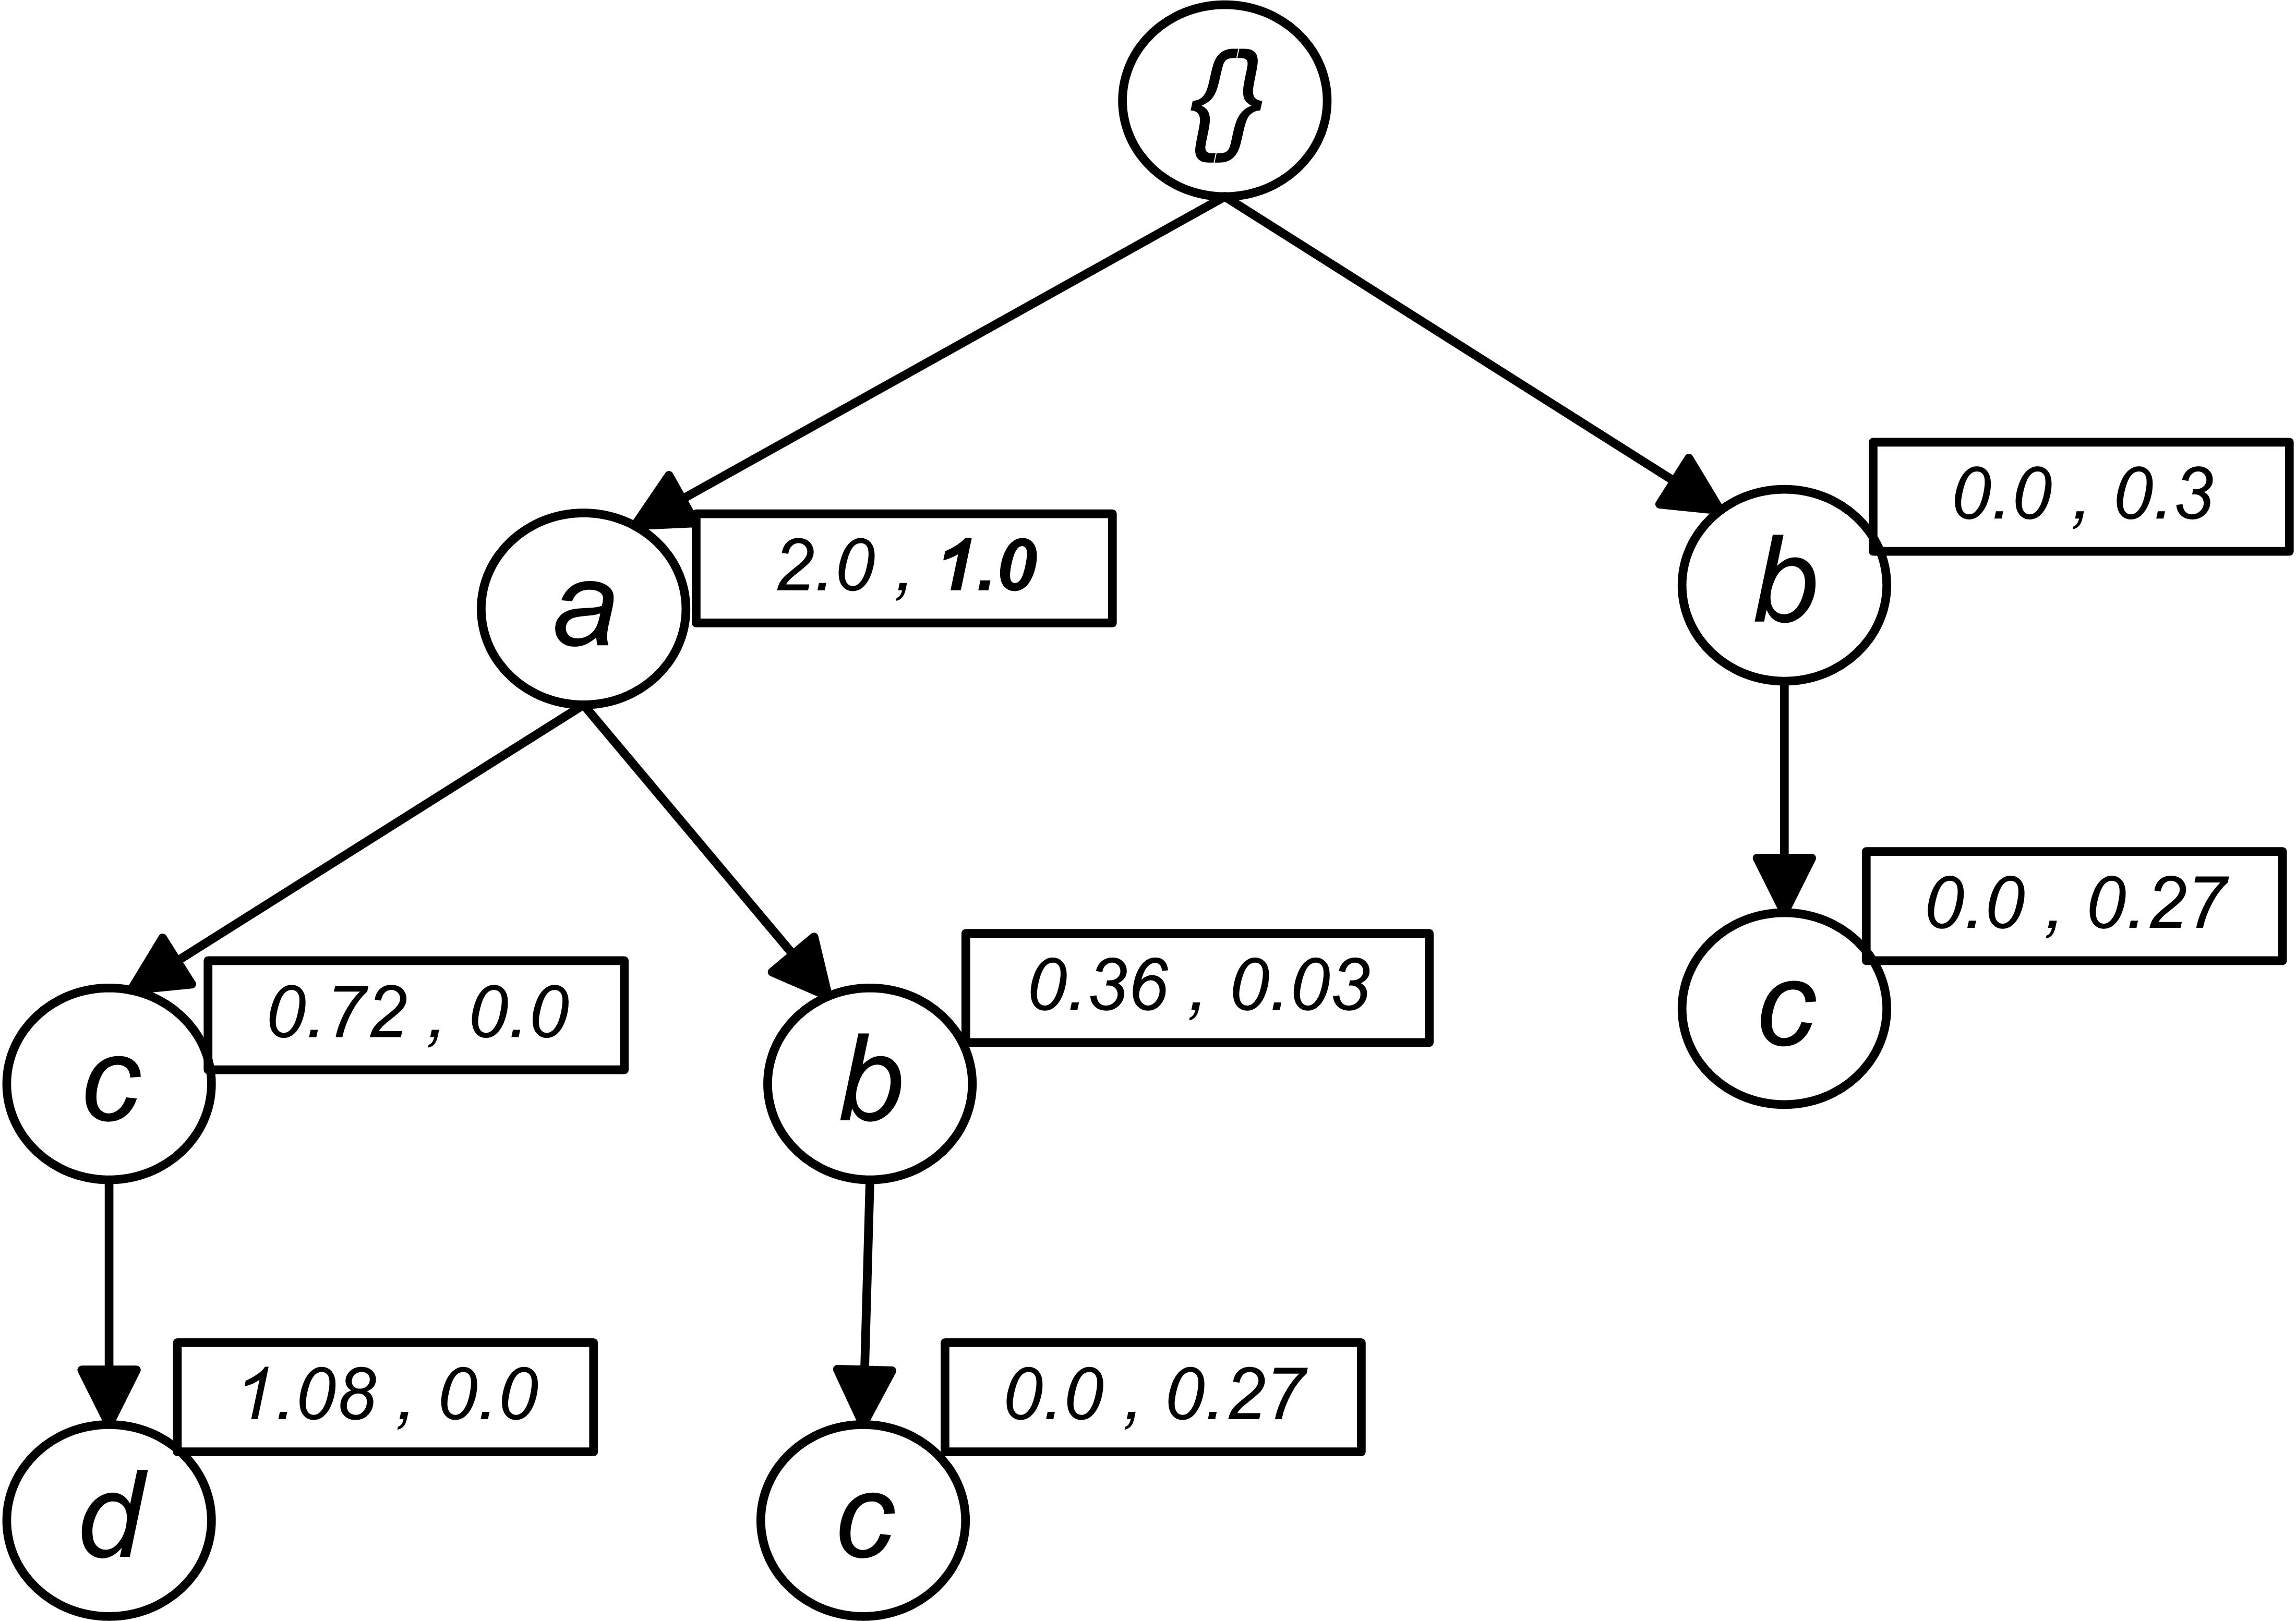
\includegraphics[width=\textwidth]{images/M_TREE.jpg}
  \captionof{figure}{US-tree for Mining}
\end{minipage}
\caption{US-tree and Header Table for Mining}
\label{figure:min_ready}
\end{figure}
%\end{document}
%\documentclass{article}
%\usepackage{caption}
%\usepackage{graphicx}
%\begin{document}
\begin{figure}
\begin{minipage}{0.40\textwidth}
  \centering
	\begin{center}
	\begin{tabular}{ |c|c| } 
 	\hline
 		Item&Value\\ \hline\hline
 		a &  1.08  	\\ \hline
 		c &  1.08   	\\ \hline
 		
\end{tabular}
\end{center}  
  \captionof{table}{\emph{d-cond tree} Header }
\end{minipage}
  \hfill
\hfill
\begin{minipage}{0.23\textwidth}
  \centering
  \hfill
  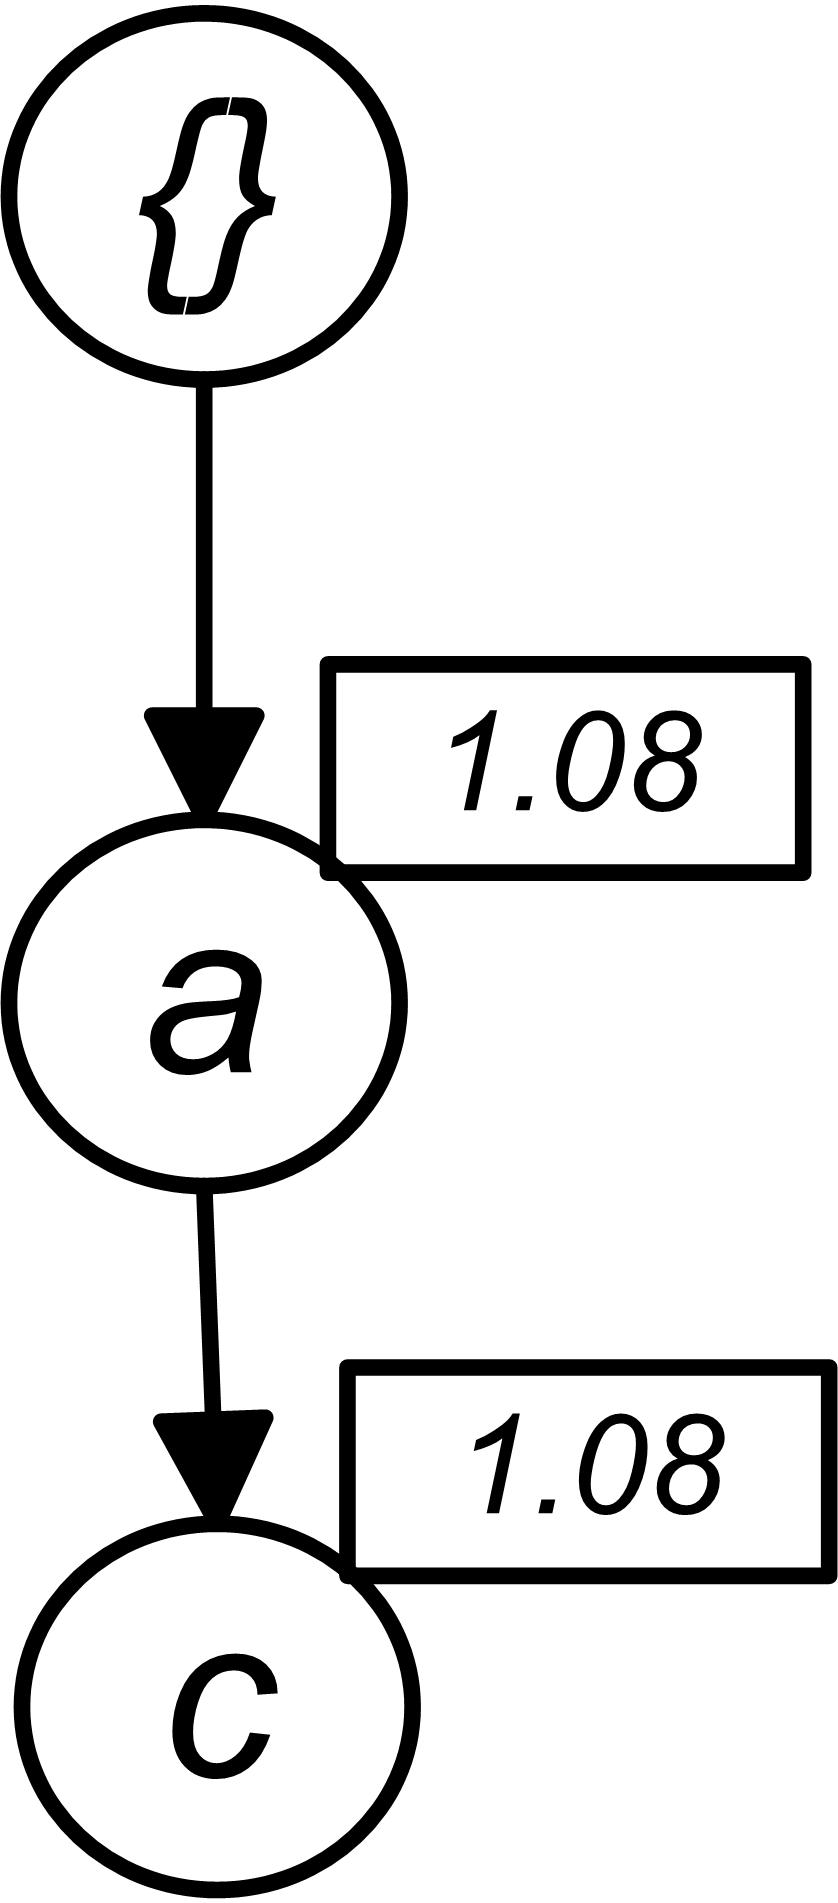
\includegraphics[width=.8\textwidth, height=5cm]{images/D_COND.jpg}
  \hfill
\end{minipage}
\hfill
\begin{minipage}{0.30\textwidth}
  \centering
  
	\begin{center}
	\begin{tabular}{ |c| } 
 	\hline
 		Freq Patterns \\ \hline\hline
 		dc  	\\ \hline
 		da   	\\ \hline
 		dca   	\\ \hline
 		
\end{tabular}
\end{center}  
  \captionof{table}{ \emph{Frequent Patterns} }
\end{minipage}
\caption{\emph{d-cond} Tree and corresponding Header}
\label{figure:d_cond}
\end{figure}
\begin{figure}
\begin{minipage}{0.30\textwidth}
  \centering
	\begin{center}
	\begin{tabular}{ |c|c| } 
 	\hline
 		Item&Value\\ \hline\hline
 		a &  .99  	\\ \hline
 		b &  .54   	\\ \hline
\end{tabular}
\end{center}  
  \captionof{table}{Header }
\end{minipage}
  \hfill
\begin{minipage}{0.29\textwidth}
  \centering
  \hfill
  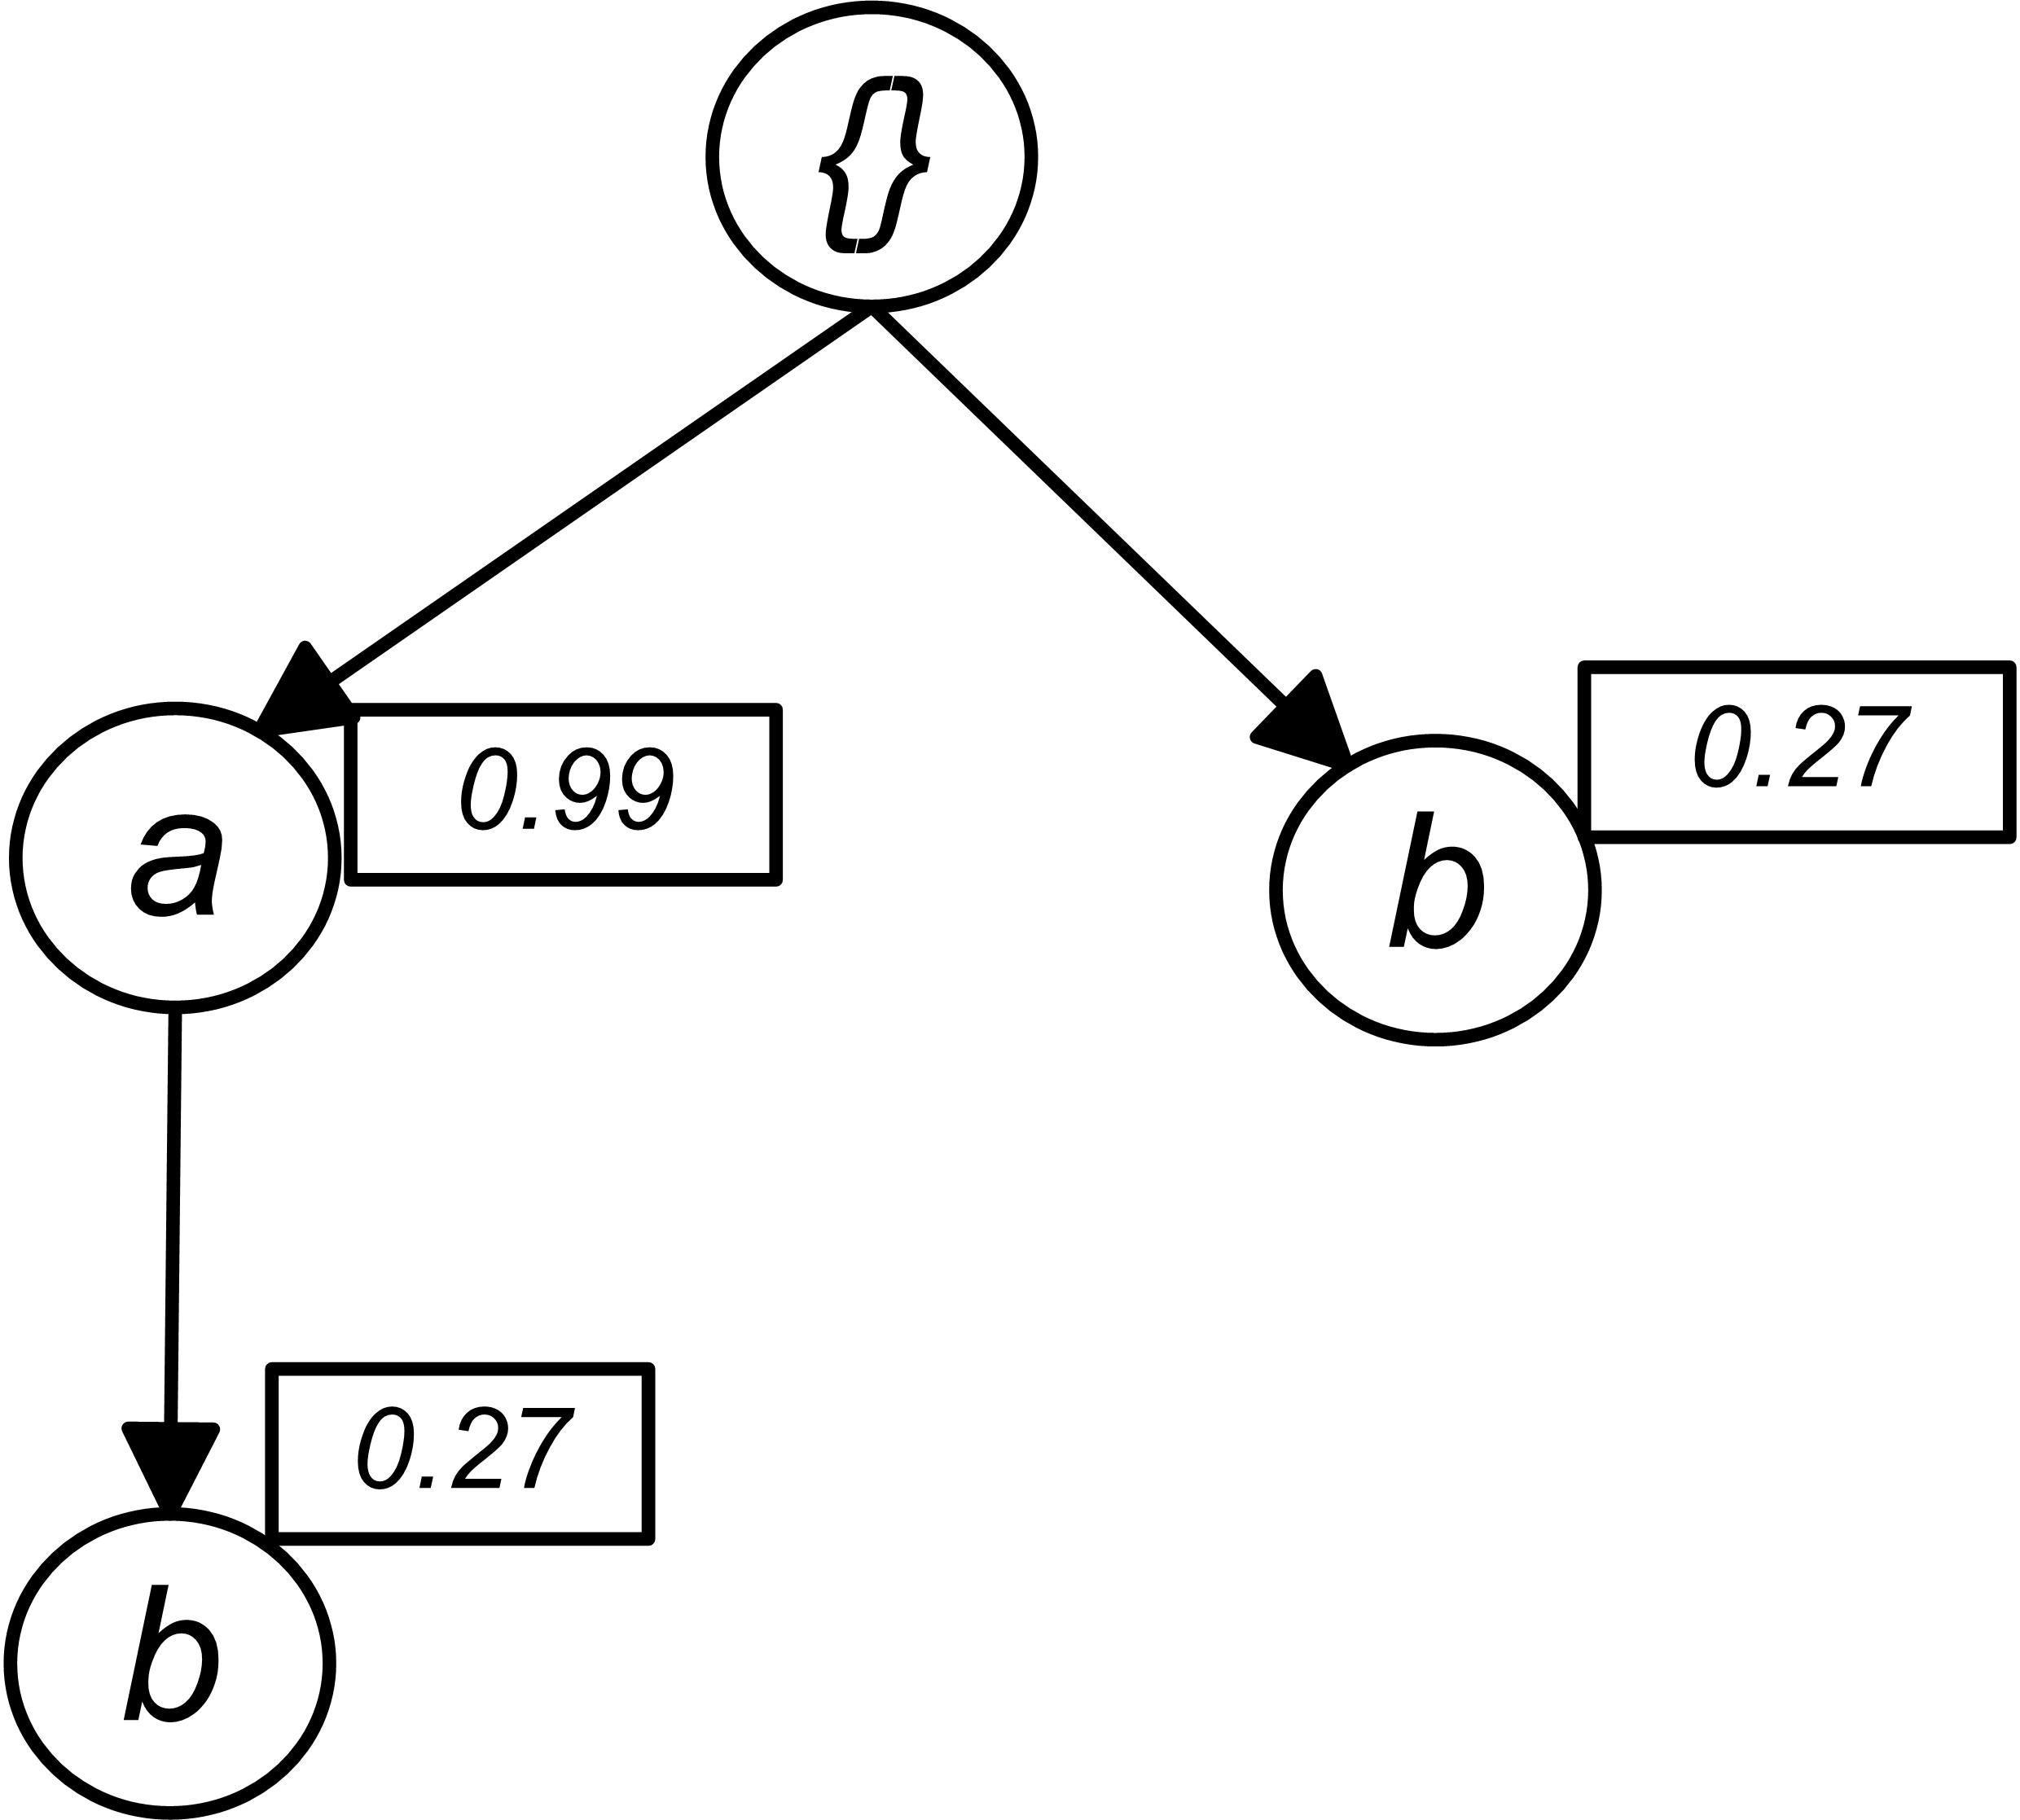
\includegraphics[width=.8\textwidth, height=3.5cm]{images/C_COND.jpg}
  \hfill  
\end{minipage}
\hfill
\begin{minipage}{0.30\textwidth}
  \centering  
	\begin{center}
	\begin{tabular}{ |c| } 
 	\hline
 		Freq Patterns \\ \hline\hline
 		ca  	\\ \hline
 		
\end{tabular}
\end{center}   
  \captionof{table}{ \emph{Freq Patterns} }
\end{minipage}
\caption{\emph{c-cond} Tree and corresponding Header}
\label{figure:c_cond}
\end{figure}
\begin{figure}
\centering
  
\includegraphics[width=.10\textwidth, height=1.1cm]{images/A_COND.jpg}
\caption{\emph{a-cond} Tree}
\label{figure:a_cond}
\end{figure}

%\end{document}

%\end{document}